
\section{Ausbildungsrufzeichen}
\label{section:ausbildungsrufzeichen}
\begin{frame}%STARTCONTENT

\begin{columns}
    \begin{column}{0.48\textwidth}
    
\begin{figure}
    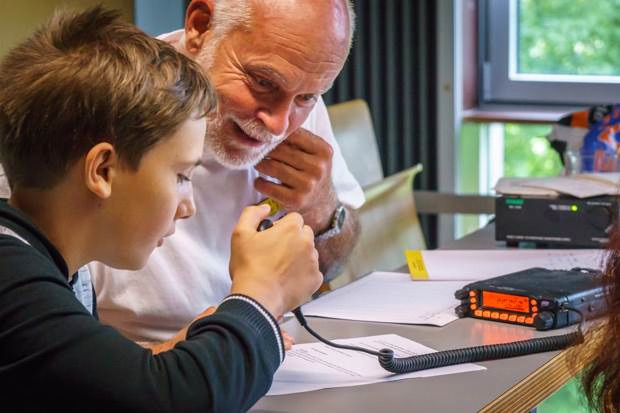
\includegraphics[width=0.85\textwidth]{foto/57}
    \caption{\scriptsize Ausbildungsfunkbetrieb verbindet oft die Generationen}
    \label{n_ausbildungsrufzeichen_ausbildungsfunkbetrieb}
\end{figure}

    \end{column}
   \begin{column}{0.48\textwidth}
       \begin{itemize}
  \item Funkamateure der Klasse~E und A sind automatisch Ausbilder
  \item Unter Aufsicht
  \item Im Berechtigungsumfang des Ausbilders
  \item Personengebundenes Rufzeichen + \enquote{/T} bzw. \enquote{/Trainee}
  \item Klubstation + \enquote{/T} bzw. \enquote{/Trainee}
  \end{itemize}

   \end{column}
\end{columns}

\end{frame}

\begin{frame}
\only<1>{
\begin{QQuestion}{VD302}{Unter welcher Voraussetzung nach der Amateurfunkverordnung (AFuV) darf ein Funkamateur Ausbildungsfunkbetrieb durchführen?}{Nur wenn er Inhaber einer Zulassung zur Teilnahme am Amateurfunkdienst der Klasse A ist}
{Wenn er Inhaber einer Zulassung zur Teilnahme am Amateurfunkdienst der Klasse A oder E ist}
{Nur wenn er mindestens 1 Jahr lang Inhaber einer Zulassung zur Teilnahme am Amateurfunkdienst ist}
{Wenn er eine gültige Rufzeichenzuteilung für ein Ausbildungsrufzeichen besitzt}
\end{QQuestion}

}
\only<2>{
\begin{QQuestion}{VD302}{Unter welcher Voraussetzung nach der Amateurfunkverordnung (AFuV) darf ein Funkamateur Ausbildungsfunkbetrieb durchführen?}{Nur wenn er Inhaber einer Zulassung zur Teilnahme am Amateurfunkdienst der Klasse A ist}
{\textbf{\textcolor{DARCgreen}{Wenn er Inhaber einer Zulassung zur Teilnahme am Amateurfunkdienst der Klasse A oder E ist}}}
{Nur wenn er mindestens 1 Jahr lang Inhaber einer Zulassung zur Teilnahme am Amateurfunkdienst ist}
{Wenn er eine gültige Rufzeichenzuteilung für ein Ausbildungsrufzeichen besitzt}
\end{QQuestion}

}
\end{frame}

\begin{frame}
\only<1>{
\begin{QQuestion}{BD211}{DG2RON führt Ausbildungsfunkbetrieb in Morsetelegrafie oder mit digitalen Übertragungsverfahren durch. Welches Rufzeichen hat der Auzubildende zu verwenden?}{DG2RON/A}
{T/DG2RON}
{DG2RON/T}
{A/DG2RON}
\end{QQuestion}

}
\only<2>{
\begin{QQuestion}{BD211}{DG2RON führt Ausbildungsfunkbetrieb in Morsetelegrafie oder mit digitalen Übertragungsverfahren durch. Welches Rufzeichen hat der Auzubildende zu verwenden?}{DG2RON/A}
{T/DG2RON}
{\textbf{\textcolor{DARCgreen}{DG2RON/T}}}
{A/DG2RON}
\end{QQuestion}

}
\end{frame}

\begin{frame}
\only<1>{
\begin{QQuestion}{VD304}{Was ist unter anderem im Zusammenhang mit der Durchführung von Ausbildungsfunkverkehr zu beachten? Der Ausbildungsfunkbetrieb darf~...}{nur mit einer maximalen Strahlungsleistung von \qty{10}{\W} EIRP durchgeführt werden.}
{nicht in Morsetelegrafie durchgeführt werden.}
{nur im Berechtigungsumfang der Rufzeichenzuteilung des Ausbilders durchgeführt werden.}
{nur an einer Klubstation durchgeführt werden.}
\end{QQuestion}

}
\only<2>{
\begin{QQuestion}{VD304}{Was ist unter anderem im Zusammenhang mit der Durchführung von Ausbildungsfunkverkehr zu beachten? Der Ausbildungsfunkbetrieb darf~...}{nur mit einer maximalen Strahlungsleistung von \qty{10}{\W} EIRP durchgeführt werden.}
{nicht in Morsetelegrafie durchgeführt werden.}
{\textbf{\textcolor{DARCgreen}{nur im Berechtigungsumfang der Rufzeichenzuteilung des Ausbilders durchgeführt werden.}}}
{nur an einer Klubstation durchgeführt werden.}
\end{QQuestion}

}
\end{frame}

\begin{frame}
\only<1>{
\begin{QQuestion}{BD210}{An der Klubstation DL0MOL soll Ausbildungsfunkbetrieb stattfinden. Darf der Auszubildende das Rufzeichen der Klubstation verwenden?}{Nein, es ist das persönliche Rufzeichen des Ausbilders zu verwenden.}
{Ja, wenn T/DL0MOL bzw. Trainee/DL0MOL verwendet wird.}
{Ja, wenn DL0MOL/T bzw. DL0MOL/Trainee verwendet wird.}
{Nein, an Klubstationen darf nicht ausgebildet werden.}
\end{QQuestion}

}
\only<2>{
\begin{QQuestion}{BD210}{An der Klubstation DL0MOL soll Ausbildungsfunkbetrieb stattfinden. Darf der Auszubildende das Rufzeichen der Klubstation verwenden?}{Nein, es ist das persönliche Rufzeichen des Ausbilders zu verwenden.}
{Ja, wenn T/DL0MOL bzw. Trainee/DL0MOL verwendet wird.}
{\textbf{\textcolor{DARCgreen}{Ja, wenn DL0MOL/T bzw. DL0MOL/Trainee verwendet wird.}}}
{Nein, an Klubstationen darf nicht ausgebildet werden.}
\end{QQuestion}

}
 \end{frame}

\begin{frame}
\frametitle{Ausbildungsfunkbetrieb ist …}
\begin{itemize}
  \item für Personen ohne Besitz eines entsprechenden Amateurfunkzeugnisses
  \item nicht für Aussendungen des Ausbilders selbst
  \item die praktische Vorbereitung auf das Ablegen der fachlichen Prüfung
  \end{itemize}
\end{frame}

\begin{frame}
\only<1>{
\begin{QQuestion}{VD301}{Wozu dient der Ausbildungsfunkbetrieb gemäß Amateurfunkverordnung (AFuV)? Er dient~...}{der alleinigen Vorführung des Amateurfunkbetriebes.}
{der praktischen Vorbereitung auf das Ablegen der fachlichen Prüfung zum Erwerb eines Amateurfunkzeugnisses.}
{der Teilnahme des Auszubildenden am Amateurfunkdienst ohne Aufsicht.}
{der Vervollständigung der Fertigkeiten des Funkamateurs in der Morsetelegrafie.}
\end{QQuestion}

}
\only<2>{
\begin{QQuestion}{VD301}{Wozu dient der Ausbildungsfunkbetrieb gemäß Amateurfunkverordnung (AFuV)? Er dient~...}{der alleinigen Vorführung des Amateurfunkbetriebes.}
{\textbf{\textcolor{DARCgreen}{der praktischen Vorbereitung auf das Ablegen der fachlichen Prüfung zum Erwerb eines Amateurfunkzeugnisses.}}}
{der Teilnahme des Auszubildenden am Amateurfunkdienst ohne Aufsicht.}
{der Vervollständigung der Fertigkeiten des Funkamateurs in der Morsetelegrafie.}
\end{QQuestion}

}
\end{frame}

\begin{frame}
\frametitle{Ausbilder …}
\begin{itemize}
  \item muss in unmittelbarer Nähe des Auszubildenden sein
  \item bei Bedienung und Betriebsabwicklung anleiten
  \item schaltet den Sender im Extremfall ab
  \item muss auf Verlangen der BNetzA Auskunft über \enquote{Art und Umfang} des Ausbildungsbetriebs geben
  \end{itemize}

\end{frame}

\begin{frame}
\only<1>{
\begin{QQuestion}{VD305}{Was ist bei der Durchführung von Ausbildungsfunkverkehr zu beachten?}{Der Ausbildungsfunkverkehr darf ausschließlich in Telefonie (SSB oder FM) durchgeführt werden.}
{Beim Ausbildungsfunkverkehr darf nicht an Amateurfunkwettbewerben teilgenommen werden.}
{Der Ausbildungsfunkverkehr darf ausschließlich in Gegenwart des Ausbilders an einer Klub- oder Schulstation durchgeführt werden.}
{Der  Ausbilder  hat  auf  Verlangen  der  Bundesnetzagentur  Auskunft  über  Art  und  Umfang  des 
Ausbildungsfunkbetriebs zu geben.}
\end{QQuestion}

}
\only<2>{
\begin{QQuestion}{VD305}{Was ist bei der Durchführung von Ausbildungsfunkverkehr zu beachten?}{Der Ausbildungsfunkverkehr darf ausschließlich in Telefonie (SSB oder FM) durchgeführt werden.}
{Beim Ausbildungsfunkverkehr darf nicht an Amateurfunkwettbewerben teilgenommen werden.}
{Der Ausbildungsfunkverkehr darf ausschließlich in Gegenwart des Ausbilders an einer Klub- oder Schulstation durchgeführt werden.}
{\textbf{\textcolor{DARCgreen}{Der  Ausbilder  hat  auf  Verlangen  der  Bundesnetzagentur  Auskunft  über  Art  und  Umfang  des 
Ausbildungsfunkbetriebs zu geben.}}}
\end{QQuestion}

}
 \end{frame}%ENDCONTENT
